\section{Generación de tablas de enclavamiento}

	\label{sec:rutas}
	
	% Once the signalling is generated and simplified, it is necessary to establish the railway routes to create the railway interlocking table. A railway route is the simplest path between two consecutive signals in the same direction, using the same tracks \cite{SIGNALLING_1,AUTOMATIC_SIMPLE_SIGNAL}. The route may contain switches, level crossings, platforms or any railway element within the path. A railway route is defined with a start and an end signal, accompanied by the indication of the corresponding safe state of the railway netElements like switches or level crossings and the tracks assigned (P1, P2, P3, P4, P5, P6, P7). Algorithm \ref{alg:routes} describes the mechanisms to detect and assign routes.
	
	\lipsum[1-5]
	
	\begin{algorithm}[hbt!]
        \caption{Route detection algorithm}\label{alg:routes}
        \DontPrintSemicolon
        %\SetAlgoLined
        \SetNoFillComment
        \LinesNotNumbered 
        Routes = []\; 
        route = 0\;
        \For{ start in [Signals] }
        {
            \tcc{Find manoeuvre and circulation signals}
            \If{ start != "Stop" }
            {
                dir = start\_sig.Direction\;
                \tcc{Find next signal w/ same direction}
                
                end = find\_next\_signal(start,[Signals])\;

                [paths] = find(start.node,end.node,graph)\;
                
                \For{ node in [paths] }
                {
                    \tcc{Find rail objects within path}
                    sws = find(graph[node],switches)\;
                    lc = find(graph[node],levelCrossings)\;
                    ptf = find(graph[node],platforms)\;
                    %route ++\;
                    Routes[route++] = $\{$start,end,dir,node,sws,lc,ptf$\}$\;
                }
            }
        }
        \KwResult{[Routes]} 
    \end{algorithm}
    
    %Stop signals cannot be starting signals and, therefore, are ignored, considering only circulation and manoeuvre signals. It is necessary to follow the graph network in the same direction as the starting signal to identify all the incoming signals through all the possible paths from the netElement where the starting signal is. For example, three routes were highlighted in Figure \ref{fig:Routes} over the simplified signalling for Example 1, with signal S22 as the starting signal: S22 to S32, S22 to X15 and S22 to T05.
    
    \lipsum[1-2]
    
    \begin{figure}[h]
    	\centering
    	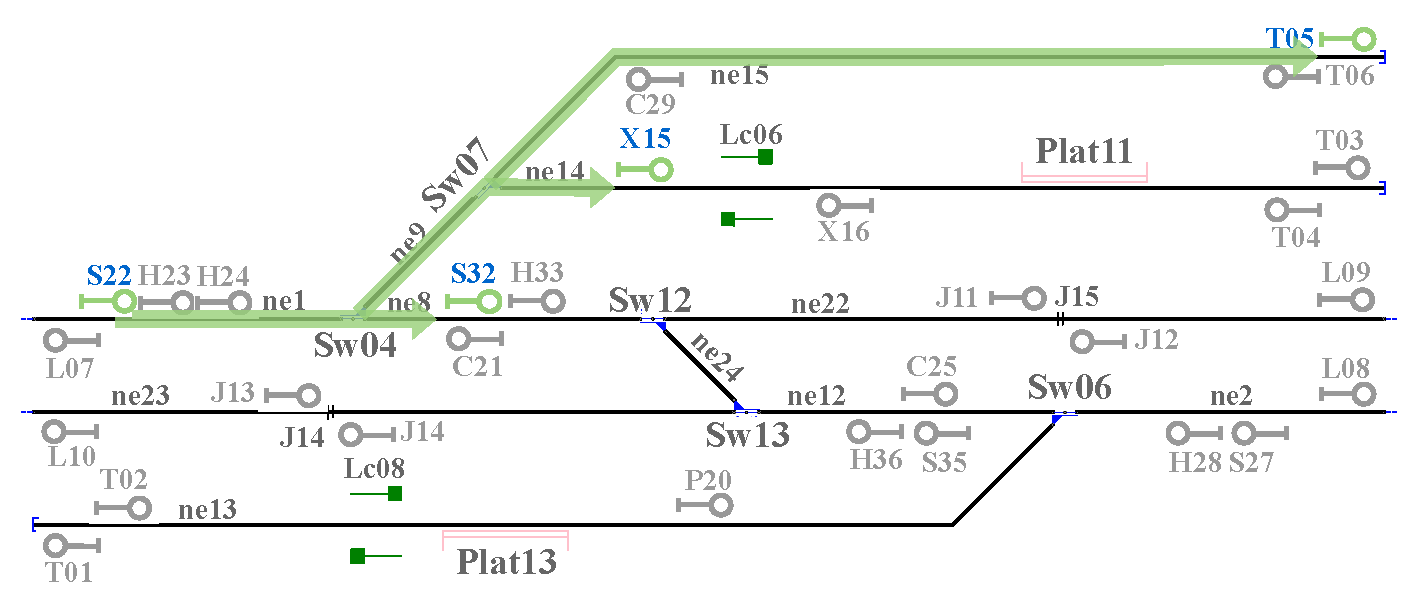
\includegraphics[width=1\textwidth]{Figuras/Figure11.pdf}
    	\centering\caption{Signalling simplified in Example 1 with three routes indicated.}
    	\label{fig:Routes}
    \end{figure}
    
    %Having the start signal and all the end signals, it is necessary to identify the main rail objects within those paths, such as switches (their position), level crossings (that must be closed), platforms and tracks. In Example 1 (Figure \ref{fig:Routes}), a route defined by signals S22 and T05 covers tracks ne1, ne9 and ne15 using switch Sw04 in reverse position and switch Sw07 in normal position without any level crossing is involved.
    
    %If two routes share the same start signal or end signal they are conflicting routes. The same if they share one netElement, switch, level crossing or the same signals swapped. It means both routes cannot be approved at the same time, one of them being approved implies the others must be blocked until the first one was completed or cancelled. Two routes could have the same start and end signal but use different tracks, but they cannot be approved at the same time because there must be necessary a switch within that routes, with opposite positions and only one position can be approved when one route is ongoing. Conflicting routes are indicated in the interlocking table that is automatically generated by the RNA. Every route is created based on the created graph network and the shortest path algorithm for directed graphs. The paper \cite{GRAPH_4_ROUTES} explores another approach to finding routes based on interlocking tables.
    
    \lipsum[1-3]